\subsubsection{Kop v štandardnej lige robotov}\label{sec_bremen}
V tejto časti popíšeme prístupy vykonávania kopov robotov, ktoré boli vytvorené mimo simulovanej 3D ligy. Predlohou simulovanej ligy je robot, ktorý je primárne určený pre štandardnú ligu. Pričom princípy prostredia a pohyby robota sú podobné. 

V práci \cite{bremen} opisujú spôsob, ako vykonávať dynamický kop. Dynamické vykonanie kopu do lopty vychádzalo zo starších prístupov na dynamickú chôdzu. Na výpočet dráhy končatiny opäť použili Bezierove krivky tretieho stupňa. Avšak tentoraz je ich pohyb založený na sekvencii týchto kriviek za sebou. Konkrétne fáza kopu je rozdelená na 7 častí - pristavenie robota k lopte, nadvihnutie chodila, náprah, kopnutie do lopty, nastavenie nohy na pôvodné miesto, spustenie chodidla k zemi a vyrovnanie kĺbov na pôvodné pozície. Schému kopu zobrazuje obrázok \ref{pic_kick_arch_bremen}. 

Krivky pohybu sú vypočítané na základe vstupných parametrov pre kop. Parametrami sú pozícia pre umiestnenie lopty, smer pohybu, číslo fázy a názov končatiny. Z opísaných častí pohybu je možné počas vykonávania meniť náprah a kopnutie do lopty, ktoré sa vie prispôsobiť na základe situácie v čase vykonávania kopu.

Pohyb sa skladá z viacerých pospájaných kriviek v určitých bodov. To má svoju nevýhodu, že ak sú takéto krivky pospájané nedávajú spojitú krivku. Výsledná krivka by mala byť vytvorená tak, aby pohyb bol plynulý bez nejakého prerušenia alebo zaseknutia. 

\begin{figure}[H]
	\center
	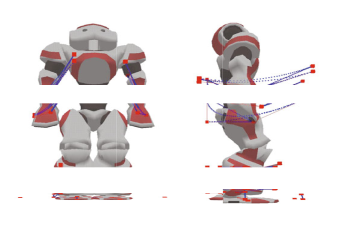
\includegraphics[scale=1]{./data/kick_arch_bremen}
	\caption{Vizualizácia kopu \cite{bremen}}
	\label{pic_kick_arch_bremen}
\end{figure}

Spojiť viac kriviek v spoločnom bode je jednoduchá záležitosť. Avšak takáto krivka nie je derivovateľná vo všetkých bodoch. Deriváciu nemá definovanú práve v spoločnom bode. V článku uvádzajú aj spôsob, za ktorých podmienok je možné dosiahnuť spojitú funkciu. V simulovanej lige nie je potrebné dodržiavať podmienky derivovateľnosti spojených kriviek, pretože pohyby robota prebiehajú vo fázach.

Stabilitu dosiahli implementovali ako samostatný modul. Pre stabilizovanie robota pri kope využili jeho ťažisko. Ťažisko smeruje vždy do zeme a jeho pozíciu umiestňujú do stredu vyvažovacieho mnohouholníka. Mnohouholník má pri kope tvar a veľkosť podpornej nohy. Výpočet je realizovaný ako harmonický priemer $n$ budúcich pozícií podpornej nohy. Vstupom do efektora, ktorý vyrovnáva náklon je rozdiel medzi aktuálnym a vypočítaným bodom ťažiska.

Ostatné externé vplyvy kompenzujú uhlovou rýchlosťou pomocou informácií z gyroskopu. % ... \textit{doplniť}